%% thesis.tex 2014/04/11 %
% Based on sample files of unknown authorship.
%
% The Current Maintainer of this work is Paul Vojta.

\documentclass[masters]{ucbthesis}
\usepackage{biblatex}
\usepackage{color}
\usepackage{graphicx}
\usepackage{siunitx}
% To compile this file, run "latex thesis", then "biber thesis"
% (or "bibtex thesis", if the output from latex asks for that instead),
% and then "latex thesis" (without the quotes in each case).

% Double spacing, if you want it.  Do not use for the final copy.
\def\dsp{\def\baselinestretch{1.5}\large\normalsize}
\dsp

% If the Grad. Division insists that the first paragraph of a section
% be indented (like the others), then include this line:
% \usepackage{indentfirst}

% Helpful commands
\newcommand{\TODO}[1]{{\color{red}\textbf{TODO: #1}}}
\newcommand{\RISCV}{\mbox{RISC-V}}
\bibliography{refs}


% Increase the depth of numbering sections

\hyphenation{Rocket-Chip}
\begin{document}

% Declarations for Front Matter

\title{An FPGA-Hosted Configurable Off-Chip Memory Model}
\author{David Thomas Biancolin}
\degreesemester{Spring}
\degreeyear{2017}
\degree{Master of Science}
\chair{Professor Krste Asanovi\'c}
\othermembers{Professor Jonathan Bachrach}
\numberofmembers{2}
% Previous degrees are no longer to be listed on the title page.
% \prevdegrees{B.A. (University of Northern South Dakota at Hoople) 1978 \\
%   M.S. (Ed's School of Quantum Mechanics and Muffler Repair) 1989}
\field{Electrical Engineering and Computer Science}
% Designated Emphasis -- this is optional, and rare
% \emphasis{Colloidal Telemetry}
% This is optional, and rare
% \jointinstitution{University of Western Maryland}
% This is optional
\campus{Berkeley}

% For a masters thesis, replace the above \documentclass line with
% \documentclass[masters]{ucbthesis}
% This affects the title and approval pages, which by default calls this
% document a "dissertation", not a "thesis".

% A slightly modified template of the ms thesis to reuse the title variables
%\makeatletter
\thispagestyle{empty}

\begin{center}
\rule{6.5in}{0.40mm}

\vspace{0.35in}
    {\large \textbf{\@title} }

\vspace{0.25in}
    {\large by \@author }

\vspace{0.35in}
\rule{6.5in}{0.40mm}

\vspace{0.5in}
    {\large {\textbf{Research Project}}}
\end{center}

\noindent Submitted to the Department of Electrical Engineering and
Computer Sciences, University of California at Berkeley,
in partial satisfaction of the requirements for the degree
of \textbf{Master of Science, Plan II}.

\vspace{0.25in}
\noindent Approval for the Report and Comprehensive Examination:

\begin{center}
    \textbf{ Committee:}

\vspace{0.25in}
\rule{3.5in}{0.25mm}

\@chair

Research Advisor

\vspace{0.25in}
\rule{3.5in}{0.25mm}

(Date)

\vspace{0.25in}
* * * * * * *

\vspace{0.25in}
\rule{3.5in}{0.25mm}

\@othermembers

Second Reader

\vspace{0.25in}
\rule{3.5in}{0.25mm}

(Date)
\end{center}
\makeatother

%\maketitle
% Delete (or comment out) the \approvalpage line for the final version.
%\approvalpage
%\copyrightpage

Recent work in FPGA-accelerated simulation of ASICs has shown that much
of a simulator can be automatically generated from ASIC RTL.  Alas, these works rely on simple models of
the outer cache hierarchy and DRAM, as
mapping ASIC RTL for these components into an FPGA fabric is too
complex and resource intensive.  To improve FPGA simulation model
accuracy, we present \PNAME~(FPGA-Accelerated Simulation and Evaluation of DRAM), a
parameterized generator of composable, high-fidelity, FPGA-hosted
last-level-cache and DRAM models. \PNAME instances are highly
performant, yet they maintain timing faithfulness independently of the
behavior of the host-FPGA memory system.
For a given scheduling policy, a single \PNAME instance can model
nearly the entire space of realizable single-channel DDR3 memory
organizations, without resynthesizing the simulator RTL.
We demonstrate \PNAME by integrating it into a flow that automatically
transforms RTL for multicore RISC-V processors into full-system
simulators that execute at up to 150 target MHz on cloud-hosted FPGAs.


\begin{frontmatter}

% You can delete the \clearpage lines if you don't want these to start on
% separate pages.

\setcounter{tocdepth}{2}
\setcounter{secnumdepth}{2}
\tableofcontents
\clearpage
\listoffigures
\clearpage
\listoftables

\begin{acknowledgements}
\end{acknowledgements}

\end{frontmatter}

\pagestyle{headings}

% (Optional) \part{First Part}

\chapter{Introduction}
\chapter{Introduction}



\chapter{A Renewed Case for FPGA-Accelerated Simulation}
% This section describes historical and related FPGA simulation work, and aims
% to call out techniques employed by this paper, in addition to describing
% problems with those works

We first review the use of FPGAs for architecture studies.  Throughout
this paper, we make a distinction between the \emph{target} and
the \emph{host}.  The target is the design under study.  Combining the
target with a model of the environment in which it executes forms a
determinate closed system whose behavior is defined independently of
the simulation host.  The host is the hardware that
executes~(\emph{hosts}) the simulation.  In this paper, a host
consists of one or more CPUs connected to one or more FPGAs.

\section{FPGA Prototyping}
FPGAs have long been used to \emph{prototype} ASICs by implementing
the ASIC RTL directly in FPGA logic.  While FPGA prototypes are both
fast~(10s to 100s of MHz) and detailed, they require a complete RTL
description of the target design. Furthermore, larger designs must be
painstakingly partitioned across multiple FPGAs. Since these
multi-FPGA prototypes advance in lockstep, cycle by cycle, they are
considerably slower~(100s of KHz to 1s of MHz). Nonetheless, FPGAs are used widely
in industry, as they allow software development and hardware
validation to proceed months before silicon is available.

\section{FPGA-Accelerated Simulation}

Prior work has explored techniques to make FPGAs more usable and
powerful simulation hosts.  Motivated by the dawn of the multicore
era, the multi-university RAMP project~\cite{RAMP} made large strides
in improving FPGA-accelerated simulators by improving resource
efficiency, developing FPGA partitioning techniques, and avoiding FPGA
recompilation by using reconfigurable models.

ProtoFlex~\cite{protoflex} was an architecture-level simulator that
demonstrated 16-way host-multithreading of a single FPGA-hosted functional model.
ProtoFlex could switch between FPGA-hosted and CPU-hosted modes via
\emph{transplantation}. FAST~\cite{FAST}, a cycle-accurate simulator, was
split into CPU-hosted functional and FPGA-hosted timing models.  RAMP
Gold~\cite{RAMPGold} used FPGA-hosted timing and functional models
with 64-way host-multithreading to model a larger target on a single
FPGA.  HAsim~\cite{HASIM} also used FPGA-hosted timing and functional
models, but provided more detailed pipeline and memory hierarchy
models.

Other work studied partitioning targets over multiple FPGAs.
\cite{LIFPGADesign} showed that by partitioning HAsim over two FPGAs, they
could model eight times as many cores, due to improved resource sharing between
virtual instances. To model a datacenter-scale target, DIABLO~\cite{Diablo}
leveraged RAMP Gold's multithreading to simulate 3072 servers on 24 FPGAs.

A unifying theme of FPGA-accelerated simulators is that one clock-cycle of
target time is executed over a variable number of FPGA-host
cycles.  This lets an FPGA-hosted simulator hide
variable host latencies to DRAM and CPU-hosted components, enables
optimizations that trade host time for host resources, and, crucially,
facilitates deterministic simulation.  This \emph{host-target
decoupling} is what differentiates an FPGA-accelerated simulator from
an FPGA prototype. We expand on this property in
Section~\ref{sec:fame1}.

\section{Adoption Challenges}

Despite their promise, FPGA-accelerated simulators have only been
successfully employed by those who designed them. We attribute their
limited appeal to several factors:

\begin{enumerate}

    \item \textbf{Availability.} Much of the early FPGA-accelerated
    simulator research relied on boutique FPGA-emulation
    platforms or custom board designs, whose high cost and
    limited availability prevented adoption.

    \item \textbf{FPGA Capacity.} Common ASIC structures, such as CAMs and
        multi-ported RAMs, map poorly to FPGA
        fabrics~\cite{FPGAGap2}, making it difficult to host large
        ASIC designs on FPGAs.

    \item \textbf{Ease of Use.} To avoid partitioning across multiple
     FPGAs, previous work focused on efficiently mapping more of the
     target to a single FPGA. The abstract, multithreaded models these
     simulators typically employ can be more difficult to implement
     than the machines they model, greatly undermining their
     usability. This complexity limits configurability, forcing users
     to modify a sophisticated piece of RTL to make larger
     changes. Furthermore, these abstract models must, like their
     software counterparts, be validated and calibrated, making them
     even more laborious to use.
\end{enumerate}

\section{Recent Technological Advances}

Even as Moore's law wanes, FPGA capacity continues to scale. The largest FPGAs
have over \wunits{50}{MiB} of BRAM and millions of logic cells.
%\footnote{Scaling RAMP
%Gold~\cite{RAMPGold} to use the largest Xilinx UltraScale+
%FPGA~\cite{Ultrascale} would permit modeling more than 5000 cores!}
As they
have scaled, FPGAs have become more heterogeneous, adding features that make
them better hosts for full-system simulators.  Both Intel and Xilinx sell FPGAs
with embedded microprocessors, making it easier to co-simulate tightly coupled
hardware and software models. Modern FPGAs include dedicated DRAM
controllers that support memory bandwidths rivaling those of ASICs.

Lower cost and increased on-chip integration have also made FPGAs more
accessible to researchers.  Not only are commercial off-the-shelf development
boards cheaper and more full-featured, FPGAs are now available as a cloud service~\cite{amazonf1}.
Where in the past academics would have to purchase their own FPGAs to reproduce
published experiments, instead, it is now possible to spin up identical
simulations on FPGAs in the cloud.  This development promises to foster more
collaboration around FPGA-accelerated simulation.

\section{Usability Through Automation}

While the trends described in the previous section solve the
\emph{availability} and \emph{FPGA capacity} challenges, usability remains a
problem. Previous work~\cite{fabscalarfpga, strober} has shown that much of an
FPGA-accelerated simulator can be automatically generated from source RTL. This RTL
can be written in an HDL like Verilog, generated by a high-level synthesis
tool, or emitted by languages like Chisel~\cite{Chisel} or Bluespec.

Alas, it is not always practical to generate models from source
RTL. Consider off-chip memory systems: they are too resource-intensive to host
in the FPGA fabric, yet for reasonable simulation performance, they must be
tightly coupled with the processor model.  Components like these require
an abstract model to virtualize the target memory system over DRAM attached
to the FPGA---reintroducing the problem that anything
but a simplistic model is difficult to design, validate, modify, and reuse.

To avoid these pitfalls, we propose writing detailed memory-system
timing models as decoupled, split-timing-and-functional models with
the timing models written as \emph{target-time} RTL. Using this
approach, the same RTL transformations applied automatically to the
processor RTL are applied to the timing-model RTL before binding it to
the functional model.  Model designers can focus on modeling detailed
target behavior and not worry about the mapping to the host.  With our
approach, since timing models are transformed from target-time RTL, it
is possible to use HLS-generated RTL or even existing
memory-controller RTL as a timing model.

To improve reusability, we propose writing timing models
as \emph{generators}.  This allows the model designer to describe a
space of \emph{instances} with less development effort.  To
support reconfiguring timing models without FPGA recompilation, timing
models expose timing parameters as I/Os that are bound automatically
to memory-mapped registers during timing-model generation.  Taken
together, these techniques make it possible to describe
detailed, reusable memory-system models.  We demonstrate this claim with \PNAME.


\chapter{An Overview of MIDAS}
We prototype our models in an FPGA-Accelerated simulation framework that builds on
the Rocket-Chip \cite{rocketchip} infrastructure (similar to
\cite{strober}). Our designs are developed in Chisel, a high-level
hardware-description language written in Scala. Building on this infrastructure
allows us to leverage a large amount of available open-source IP and a growing
software ecosystem that includes GCC, Linux and LLVM.

Our framework makes use of FIRRTL~\cite{firrtl}, an intermediate representation
(IR) for RTL that has frontends for both Chisel and Verilog, and can target
both FPGA and ASIC flows by emitting optimized Verilog output. FIRRTL enables
the implementation of compiler passes on top its IR framework. These passes
can, for example, apply FPGA-optimizations, add instrumentation, and
automatically produce scan chains for debugging and power
estimation\cite{strober} -- all without requiring modifications to the source
RTL.

\begin{figure}
	\centering
	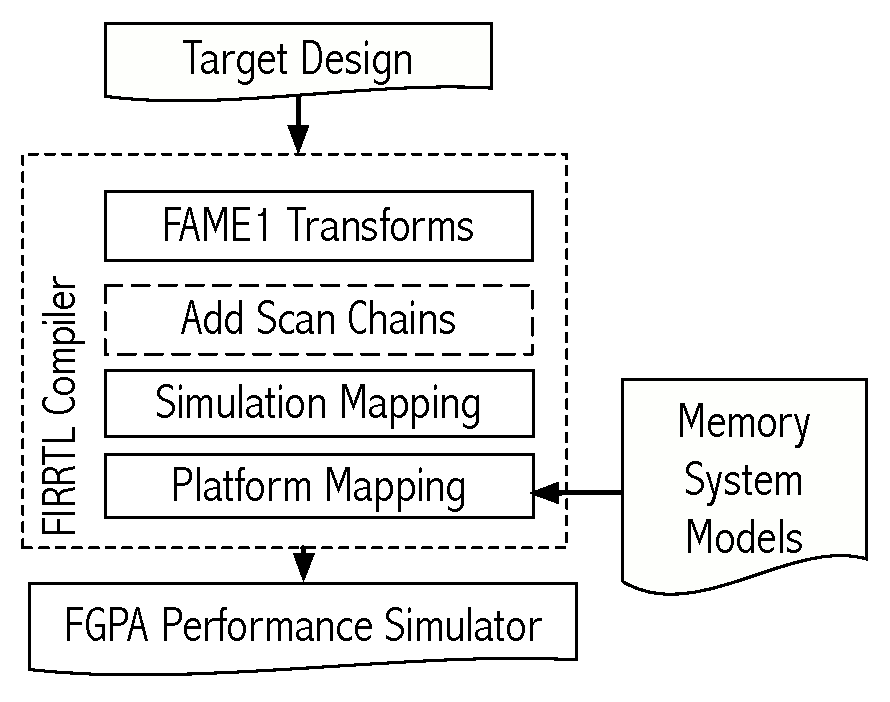
\includegraphics[width=7cm]{figures/firrtl.pdf}
	\caption{FIRRTL custom transforms for the FPGA simulator}
	\label{fig:firrtl}
\end{figure}


\section{Host-Target Decoupling in MIDAS}

\section{Transformations of Source RTL}

MIDAS uses FIRRTL compiler passes to preform transformation source RTL into
host-decoupled models. The most important of these is the FAME-1
transformation, which adds to requsite logic to host-decouple target RTL, so
that it may conform to a RAMP model of execution. \TODO{See Section}. In figure
\TODO{Auto-transformation} below, the procedure through which source RTL is
host decoupled is illustated.


Additional transformations may be invoked to add scan
chains and I/O trace buffers for debugging, and for state snapshotting for use
with Strober\cite{strober}.

\section{Platform Mapping}

\section{Target Machines}

While this approach is applicable to arbitrary RTL, one challenge lies in
sourcing the RTL to build a realistic target. While we build on RocketChip and
\RISCV, our approach could in principle be used with other open-source designs
such as OpenPiton\cite{openpiton} and FabScalar\cite{fabscalar}.


\chapter{An Overview of DRAM Off-Chip Memory Systems}
\section{DRAM Device Architecture}\label{sec:dram-arch} In a DRAM IC, arrays of
bit cells are hierarchically arranged into multiple parallel \emph{banks}.
Banks provide the primitive level of concurrency in a DRAM memory system. They
can service independent requests, assuming they do not simultaneously require
shared resources like the data, address and command buses.  Multiple DRAM ICs
can be arranged in parallel to widen the data bus; address and command buses
fan out to each IC. For more concurrency, and to support larger memory
capacities, multiple \emph{ranks} of DRAM devices may be used. Here, generally,
the command and data buses are shared between all ranks, with a one-hot
chip-select indicating which rank a command is addressed to.

A basic DRAM operation requires a series of three commands: \emph{activate
(ACT)}, \emph{column access~(CAS)}, and \emph{precharge~(PRE)}. The ACT command
enables the word-lines of the array corresponding to a single \emph{row} of the
bank. The cells of the row are sensed and saved in a \emph{row
buffer}(typically 1-2 kB). A CAS command then selects a subset of the row
buffer to read or write~(CASR and CASW commands respectively). In double-data
rate~(DDR) DRAM, data is bursted over successive rising and falling clock
edges.  While the row buffer remains \emph{open}, the row can be accessed by
issuing new CAS commands. To access a row not stored in the buffer, a PRE
command must be issued to \emph{close} the row and charge the bit lines for a
new access.

DRAM is named dynamic-RAM because it gradually loses its stored state over time
as bit-cell capacitors leak. DRAM-cell retention rates vary on a single die and
between dies and are highly sensitive to temperature~(warmer cells leak
faster). To maintain their state, DRAM cells must be periodically ``refreshed".
Activating a row of cells is sufficient to refresh them: the stored state is
read by the sense amplifiers and fed back into the bitlines at the supply
voltage, recharging the still-open capacitors.  As part of the DRAM standards,
JEDEC mandates cells must be refreshed on-average once every 8ms; an interval
they have maintained from DDR through DDR4. Since activations to every row
cannot generally be guaranteed, DRAM devices are refreshed explicitly with
a refresh command~(REF). To reduce complexity, this command refreshes a constant
number of contiguous rows beginning at a base row address in all banks
concurrently. The base address is incremented which each REF command. DRAM manufacturers generally
have kept the number of refresh commands required to iterate through the entire
array constant: 8192 commands per 8ms interval, or one on average every 64 $\mu s$.
Hence, refresh commands take longer to execute on denser devices with more rows
per bank.

A complete list of timings required to model a generic DDR protocol is give in
table \ref{tbl:dram-timings}. These have been taken, with some modification,
from \textit{Memory Systems: Cache, DRAM, Disk}\cite{drambook}.

\begin{table}[htb]
\begin{center}
\resizebox{\textwidth}{!}{%
    \begin{tabular}{|p{0.20\textwidth}|p{0.8\textwidth}|}
    \hline
    \textbf{Name} & \textbf{Description} \\
    \hline
    \hline
    \textbf{$t_{AL}$} & Additive Latency. Additional latency added to column access commands. \\
    \textbf{$t_{CAS}$~($t_{CL}$)} & Column Access Strobe latency. Delay between
    when a CASR command is received and when the first beat of read data is
    returned. \\ \textbf{$t_{CCD}$} & Column-to-Column Delay. Minimum duration
    between two consecutive column commands. \\ \textbf{$t_{CMD}$} & Command
    transport duration. The duration a command occupies the command bus. \\
    \textbf{$t_{CWD}$~($t_{WL}$)} & Column Write Delay. The delay between a
    CASW command and the when the controller must present the first beat of
    write data. \\
    \textbf{$t_{FAW}$} & Four row Activation Delay. A rolling time window
    during which only four row activations may be made to all banks of a DRAM
    device. \\
    \textbf{$t_{RAS}$} & Row Access Strobe. The minimum duration after an ACT
    command that the row must be kept open before issuing a precharge command
    to close it. \\
    \textbf{$t_{RC}$} & Row Cycle time. The minimum duration required
    to open, and close a row. $t_{RC} = t_{RAS} + t_{RP}$ \\
    \textbf{$t_{REFI}$} & Refresh Interval. The average period of time between refresh commands. \\
    \textbf{$t_{RCD}$} & Row-to-Column Delay. The minimum duration after
    activation column commands may be issued to the newly-opened row.  \\
    \textbf{$t_{RFC}$} & ReFresh Cycle time. The minimum duration after a refresh
    command that activation commands may be issued. \\
    \textbf{$t_{RP}$} & Row Precharge delay. The minimum duration after a
    precharge command that an ACT to the same bank may be issued. \\
    \textbf{$t_{RRD}$} & Row-to-Row Delay. The minimum duration between ACT commands to the same bank. \\
    \textbf{$t_{RTP}$} & Read-To-Precharge delay. The mimimum duration after a CASR command that a precharge may be issued to the same row. \\
    \textbf{$t_{RTRS}$} & Rank-To-Rank Switching delay. Accounts for time to change termination schemes on DQ and DQS buses when switching between ranks. \\
    \textbf{$t_{WR}$} & Write Recovery time. The minimum duration after a CASW command that a precharge command may be issued to the same row. \\
    \textbf{$t_{WTR}$} & Write TurnaRound Time. The minimum duration after a CASW command that a CASR may be issued to the same row. \\
    \hline
\end{tabular}}
\end{center}
\caption{A list of key timings for a conventional DDRx SDRAM}
\label{tbl:dram-timings}
\end{table}%

\clearpage
\section{DRAM Controller Architecture}

A DRAM controller is responsible for responding to memory
requests from one or more requestors by scheduling those requests over its
attached memories as a judicious stream of DRAM commands.

Memory access scheduling~(MAS) is the process by which, for a given cycle, a
controller selects a single DRAM command to be issued from a legal set. Legal
commands are constrained by the current state of each bank, the availability
of shared resources like the command and data buses, and timing constraints
imposed by the DRAM standard. Good MAS policies strike a delicate balance
between minimizing latency, maintaining quality-of-service guarantees across
multiple threads of execution, maximizing bandwidth, and minimizing power.
There are plethora of academic papers on MAS policies, and still more
industrial patents on the subject. In this work we consider two popular MAS policies. 

\subsection{First-Come First-Serve~(FCFS) Policy}\label{sec:fcfs} Commands for the
oldest pending memory reference are issued first. This is the simplest MAS
policy, but tends to under-utilize available DRAM bandwidth as younger requests
that may hit in the row-buffer are not issued before older commands that miss.
FCFS schedulers are common in older machines, and those that present few
concurrent memory requests.

\subsection{First-Ready FCFS~(FR-FCFS)~\cite{frfcfs} Policy}\label{sec:frfcfs}
First, ready~(legally issuable) column commands are prioritized over ready row
commands. Second, commands for older references are prioritized over younger
ones. This permits younger but ready column commands to be issued before older
row commands. FR-FCFS is a relatively simple scheme that improves bandwidth
utilization considerably. It is the de facto standard against which new MAS
policies for machines with a single stream of memory references~(like
single-core out-of-order machines), are compared.

\section{DRAM Software Simulation}

The current state of the art in DRAM simulation in academia are cycle-accurate
software simulators like DRAMSim2~\cite{dramsim}, Ramulator~\cite{ramulator} and
USIMM~\cite{usimm}. These models generate DRAM command streams that have been
validated against industrial models~(for some standards). Both Ramulator and
DRAMSim2 can be easily integrated into Gem5~\cite{gem5}, though gem5 includes a
detailed event-based model of its own~\cite{gem5event}. In trace-driven mode,
operating at full throughput and only as a timing-model, these cycle-accurate
models simulate at frequencies ranging from hundreds of KHz to ones of
MHz~\cite{ramulator}.

\section{DRAM Power Modeling}

In order to model power, Ramulator relies on DRAMPower~\cite{drampower}, to
which it passes its command trace. DRAMSim2 directly implements strategies
Micron has described in their technical notes~\cite{micronpower}. Micron has
also provided spreadsheets implementing these strategies, that take
microarchitectural event frequencies as input. These approaches can also be
used in an FPGA simulation, as sufficiently detailed FPGA models can add
instrumentation for specific events, while simpler models could save or sample
the memory access trace and compute power out-of-band.


% \appendix

\printbibliography

\end{document}
